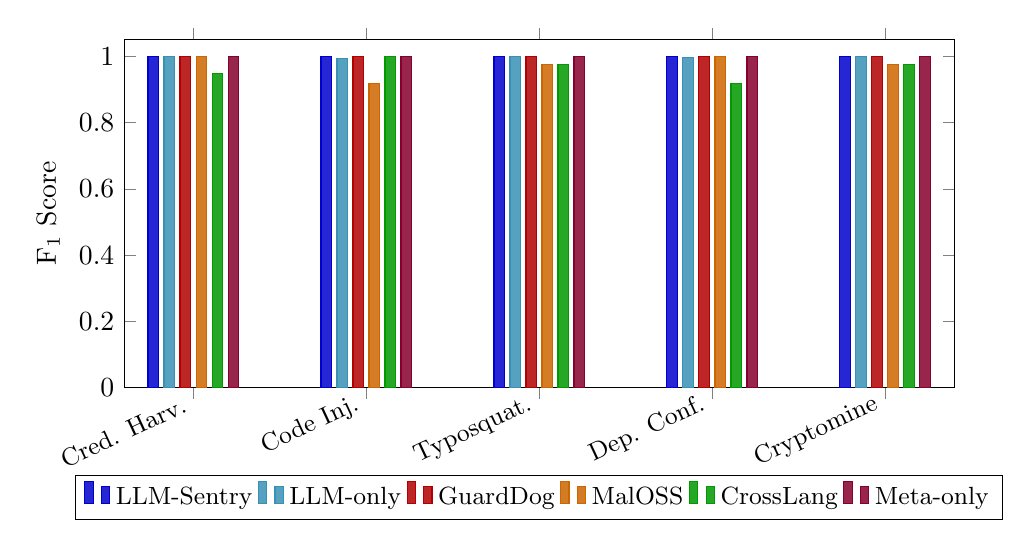
\begin{tikzpicture}
\begin{axis}[
  ybar,
  bar width=0.133cm,
  width=\linewidth,
  height=6cm,
  enlarge x limits=0.1,
  ylabel={F$_1$ Score},
  ymin=0, ymax=1.05,
  ytick={0,0.2,0.4,0.6,0.8,1.0},
  xtick=data,
  symbolic x coords={{Cred. Harv.},{Code Inj.},{Typosquat.},{Dep. Conf.},{Cryptomine}},
  x tick label style={rotate=25, anchor=east, font=\small},
  legend style={at={(0.5,-0.25)}, anchor=north, legend columns=-1,    font=\small},
  legend cell align={left},
]
\addplot[fill=blue!80!black, fill opacity=0.85, draw=blue!80!black]
  coordinates {(Cred. Harv.,1.0000) (Code Inj.,1.0000) (Typosquat.,1.0000) (Dep. Conf.,1.0000) (Cryptomine,1.0000)};
\addlegendentry{LLM-Sentry}
\addplot[fill=cyan!70!black, fill opacity=0.85, draw=cyan!70!black]
  coordinates {(Cred. Harv.,1.0000) (Code Inj.,0.9944) (Typosquat.,1.0000) (Dep. Conf.,0.9955) (Cryptomine,1.0000)};
\addlegendentry{LLM-only}
\addplot[fill=red!70!black, fill opacity=0.85, draw=red!70!black]
  coordinates {(Cred. Harv.,1.0000) (Code Inj.,1.0000) (Typosquat.,1.0000) (Dep. Conf.,1.0000) (Cryptomine,1.0000)};
\addlegendentry{GuardDog}
\addplot[fill=orange!80!black, fill opacity=0.85, draw=orange!80!black]
  coordinates {(Cred. Harv.,1.0000) (Code Inj.,0.9189) (Typosquat.,0.9744) (Dep. Conf.,1.0000) (Cryptomine,0.9744)};
\addlegendentry{MalOSS}
\addplot[fill=green!60!black, fill opacity=0.85, draw=green!60!black]
  coordinates {(Cred. Harv.,0.9474) (Code Inj.,1.0000) (Typosquat.,0.9744) (Dep. Conf.,0.9189) (Cryptomine,0.9744)};
\addlegendentry{CrossLang}
\addplot[fill=purple!70!black, fill opacity=0.85, draw=purple!70!black]
  coordinates {(Cred. Harv.,1.0000) (Code Inj.,1.0000) (Typosquat.,1.0000) (Dep. Conf.,1.0000) (Cryptomine,1.0000)};
\addlegendentry{Meta-only}
\end{axis}
\end{tikzpicture}